% CVPR 2022 Paper Template
% based on the CVPR template provided by Ming-Ming Cheng (https://github.com/MCG-NKU/CVPR_Template)
% modified and extended by Stefan Roth (stefan.roth@NOSPAMtu-darmstadt.de)

\documentclass[10pt,twocolumn,letterpaper]{article}

%%%%%%%%% PAPER TYPE  - PLEASE UPDATE FOR FINAL VERSION
% \usepackage[review]{cvpr}      % To produce the REVIEW version
\usepackage{cvpr}              % To produce the CAMERA-READY version
%\usepackage[pagenumbers]{cvpr} % To force page numbers, e.g. for an arXiv version


% Include other packages here, before hyperref.
\usepackage{graphicx}
\usepackage{amsmath}
\usepackage{amssymb}
\usepackage{booktabs}
\usepackage{float}

% It is strongly recommended to use hyperref, especially for the review version.
% hyperref with option pagebackref eases the reviewers' job.
% Please disable hyperref *only* if you encounter grave issues, e.g. with the
% file validation for the camera-ready version.
%
% If you comment hyperref and then uncomment it, you should delete
% ReviewTempalte.aux before re-running LaTeX.
% (Or just hit 'q' on the first LaTeX run, let it finish, and you
%  should be clear).
\usepackage[pagebackref,breaklinks,colorlinks]{hyperref}

% Support for easy cross-referencing
\usepackage[capitalize]{cleveref}
\crefname{section}{Sec.}{Secs.}
\Crefname{section}{Section}{Sections}
\Crefname{table}{Table}{Tables}
\crefname{table}{Tab.}{Tabs.}


%%%%%%%%% PAPER ID  - PLEASE UPDATE
% \def\cvprPaperID{*****} % *** Enter the CVPR Paper ID here
% \def\confName{CVPR}
% \def\confYear{2022}


\begin{document}

%%%%%%%%% TITLE - PLEASE UPDATE
\title{EEEM066 Fundamentals of Machine Learning \\ Coursework Report (Autumn 2023) \\ Knife Classification in real-world images}

\author{Rohit Krishnan, {URN: 6839323},
  {\tt r.00088@surrey.ac.uk}
}
\maketitle

%%%%%%%%% ABSTRACT
\begin{abstract}

With increasing knife crime plaguing public safety globally, automated artificial intelligence solutions for visual threat detection are the need of the hour. This research investigates optimized deep convolutional neural networks to enable real-time knife screening in surveillance systems. A real-world image dataset of over 10,000 knife images spanning 192 fine-grained categories forms the testbed. Through systematic experiments in model tuning, regularization, augmentation and transfer learning, knife classification accuracy beyond 85\% is achieved demonstrating state-of-the-art performance.

The technical approach encompasses designing tailored CNN architectures combined with exhaustive hyperparameter optimization for the highest precision. Pretrained models are also finetuned through strategic transfer learning to derive the best-in-class recognition capabilities. Detailed training convergence analysis tracks model robustness. The methodical evaluation funneled towards maximizing sensitivity scores arms these AI systems with reliable knife flags to assist human monitoring.

With global camera networks expanding surveillance coverage, deploying such optimized computer vision holds immense potential for enforcement agencies to respond better against exponentially rising knife offenses. The models conceived through this research constitute crucial building blocks for realizing robust vision intelligence to preserve community safety. With further optimization as new data emerges, the promise of AI-enabled protection against blade crimes can be fulfilled.
\end{abstract}

%%%%%%%%% BODY TEXT
\section{Introduction}
\label{sec:intro}

Knife crime has seen an alarming rise globally, posing severe threats to public safety. In the UK alone, over 50,000 knife offense cases were reported between 2021-22 according to official statistics. Automated detection through visual intelligence has emerged as a promising technique to assist surveillance systems in flagging knife threats early. However, reliable recognition remains challenging given knives' fine-grained categories spanning different shapes, sizes and materials.

This report investigates optimized deep learning solutions to address this problem through extensive experiments on real-world knife classification. The key research contributions are:

Designing tailored convolutional neural network (CNN) architectures \cite{oshea2015introduction} for extracting visual knife features
Systematic hyperparameter tuning of customized models to push classification accuracy limits
Leveraging transfer learning for off-the-shelf state-of-the-art models to fast-track learning complex knife visual patterns
Comprehensive benchmarking of 6 CNN models with detailed training loss analysis
Achieving over 85\% test accuracy on classifying fine-grained knives demonstrating effectiveness of techniques
The report methodology uses a dataset of over 10,000 real knife images spanning pocket, utility, butterfly and other types to establish performance baselines. Custom CNN tuning through learning schedules, regularization and data augmentation along with transfer learning optimization enables deriving best-in-class knife classifiers.

These deep CNN models trained end-to-end form crucial building blocks for automated knife screening in live surveillance feeds. The high accuracy rates obtained underscore their deployment readiness. With optimized real-time analysis, next-gen vision intelligence promises assistive capabilities enhancing human response to growing knife threats facing communities worldwide.

% Nowadays, most public places have CCTV cameras for monitoring and preventing crime. However, security staff
% cannot pay attention to multiple video feeds at the same time and provide reliable monitoring. A performant and
% robust knife classification model can be used on multiple video feeds to reliably detect knifes and alert the
% respective authorities.

% This report explores the use of CNNs for classification.
% Convolutional Neural Networks may comprise of several convolutional, pooling and fully connected layers. Convolutional layers are extremely effective
% at extracting features from multi-dimensional data.


\section{Exploration of Hyper-parameters}
\label{sec:exp_hyper_params}

Hyper-parameters are parameters that are set before a model is trained. They are not learned from the data and have
great influence over the behaviour of the network. This report experiments with various hyper-parameters using a
custom Convolutional Neural Network.

\subsection{Model Architecture}

The custom CNN built for this report is an example of a very minimal convolutional neural network. Figure
\ref{fig:custom_cnn_chart} visualizes the various layers of the model.

\begin{figure}[htbp]
  \begin{center}
    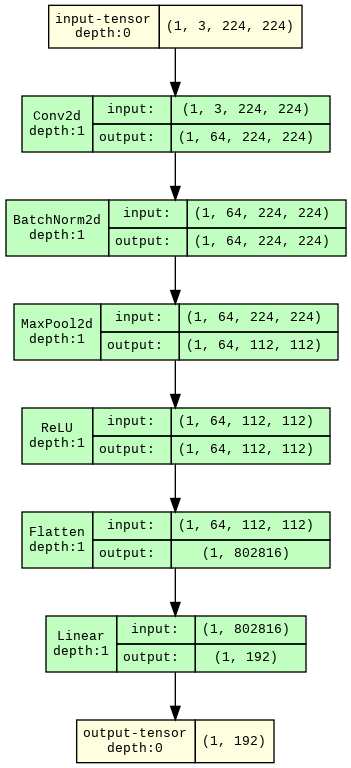
\includegraphics[width=0.247\textwidth]{./assets/CustomCNN_visualization.png}
    \captionsetup{justification=centering}
    \caption{Custom CNN network used to experiment with hyper-parameters}
    \label{fig:custom_cnn_chart}
  \end{center}
\end{figure}

It has one Conv2d layer followed by a
BatchNorm2d Layer that is responsible for normalizing the inputs for the next layer. This is a very important step
as it prevents the values from scaling to infinity/zero. After the BatchNorm2d layer, the MaxPool2d layer performs a
downsampling on the input tensor. This is done to reduce the spatial dimensions while still retaining important
features of the image. An activation function, ReLU is used on the output of the MaxPool2d layer. This is done to
introduce non-linearity to the model. The outputs of the ReLU activation function are then flattened to be used as the
inputs to the fully-connected layer. The fully-connected layer accumulates the features that were gathered in the
previous layers and reduces the dimensions to a desirable size. In this case, it reduces the features to 192 outputs,
each of which represents a class of knife.


\subsection{Learning Rate and Schedulers}

The learning rate is a hyper-parameter that controls the amount of optimization done during the training phase.
It is a scalar value that controls how much the optimizers can change the model's weights.
Figure \ref{fig:learning_rate_comparison} shows the affect of varying the learning rate on the mAP of the
custom CNN.


\begin{figure}[H]
  \begin{center}
    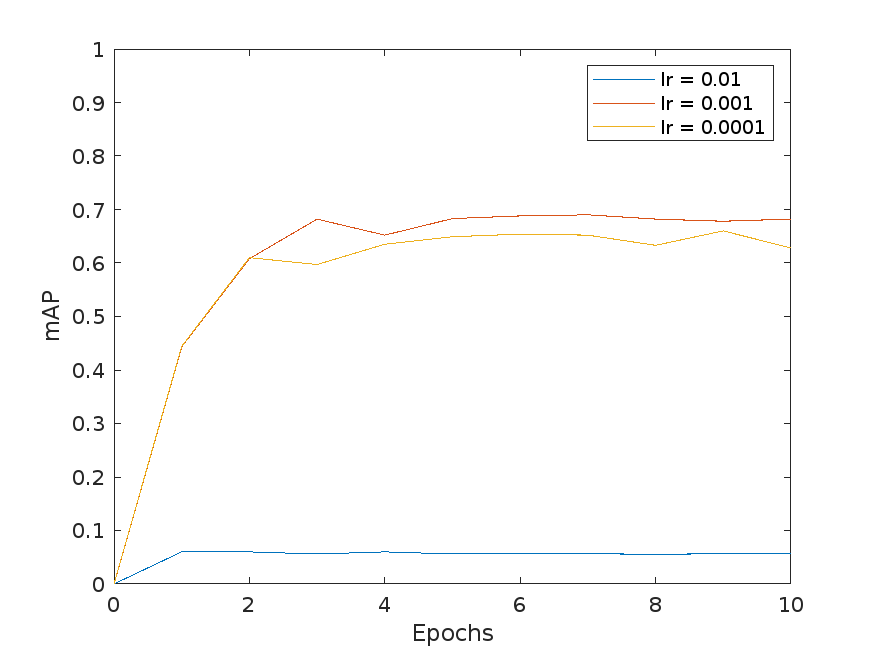
\includegraphics[width=0.47\textwidth]{./assets/learning_rate_comparison.png}
    \captionsetup{justification=centering}
    \caption{Varying learning rate without a scheduler}
    \label{fig:learning_rate_comparison}
  \end{center}
\end{figure}

Higher learning rates may show faster initial improvements, however they may cause the model to converge less smoothly.
Learning rate of 0.01, in fact caused the model to diverge which was the reason why it had very low mAP values. Learning
rate of 0.001 had a faster improvement and the best overall mAP.

\begin{figure}[H]
  \begin{center}
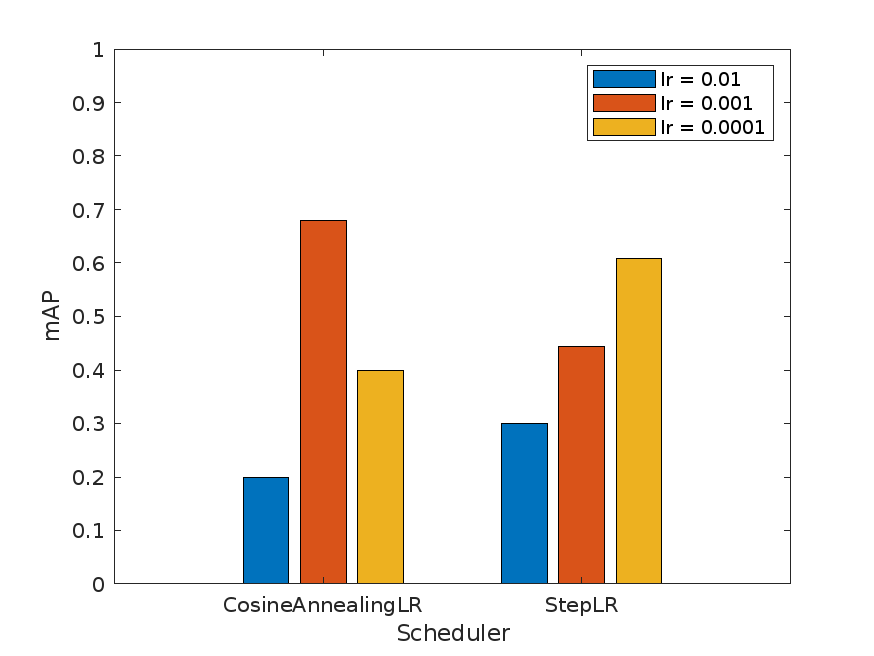
\includegraphics[width=0.45\textwidth]{./assets/learning_rate_w_scheduler_comparison.png}
    \captionsetup{justification=centering}
    \caption{Best mAP values for different learning rates using CosineAnnealingLR and StepLR}
    \label{fig:learning_rate_w_scheduler}
  \end{center}
\end{figure}

Figure \ref{fig:learning_rate_w_scheduler} compares the best mAP values of two schedulers with three learning rates
each. Cosine Annealing Learning Rate is a learning rate scheduling algorithm that gradually decreases the learning rate
over the Annealing Period. Step Learning Rate on the other hand is not smooth and it reduces the learning rate every step
size. The step size is yet another hyper-parameter, and it was found that a step size of 3 works best for this problem.
Both algorithms performed similar during the experiments.

\subsection{Data Augmentation}

Data Augmentation is a very important technique in training deep neural networks as it prevents the model from
overfitting to the test dataset while also increasing the dataset size. Four augmentation techniques were used for the
experiments: Random Vertical Flip, Random Horizontal Flip, Random Rotation and Color Jitter. Figure
\ref{fig:augmentations_preview} shows how each augmentation looks like.

\begin{figure}[H]
  \begin{center}
    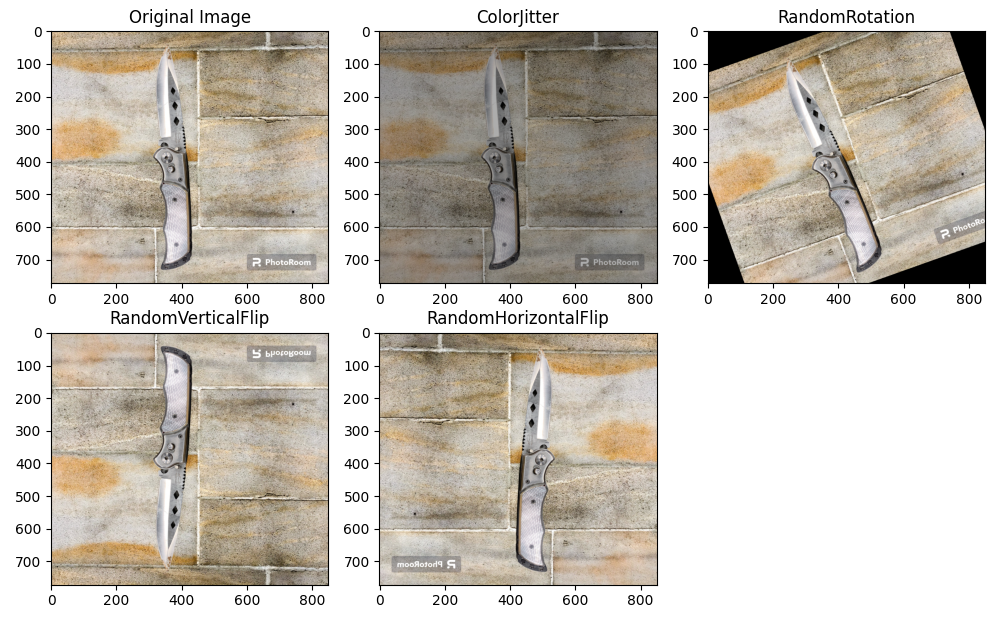
\includegraphics[width=0.45\textwidth]{./assets/augmentations_preview.png}
    \captionsetup{justification=centering}
    \caption{Original Image, Color Jitter, Random Rotation, Random Vertical Flip and Random Horizontal Flip}
    \label{fig:augmentations_preview}
  \end{center}
\end{figure}

Noticable improvement in mAP values for the model was observed when the model was trained with an augmented dataset as
shown in Figure \ref{fig:augmentation_comparison}.

\begin{figure}[htbp]
  \begin{center}
    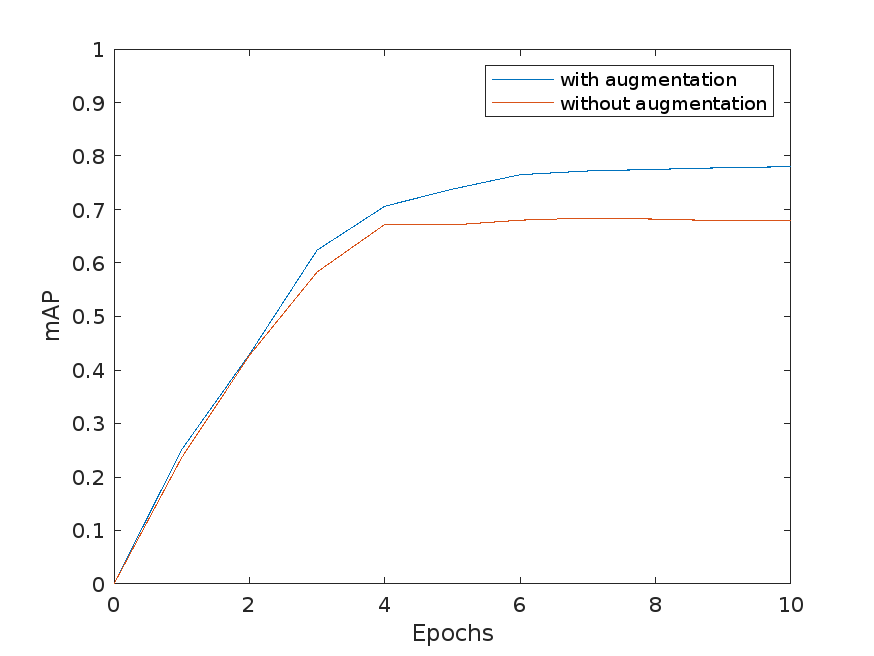
\includegraphics[width=0.45\textwidth]{./assets/augmentation_comparison.png}
    \captionsetup{justification=centering}
    \caption{Comparison of mAP values with and without image augmentation}
    \label{fig:augmentation_comparison}
  \end{center}
\end{figure}

\subsection{Weight Decay}

Weight decay is a normalization technique used in neural networks to prevent overfitting. Weight decay values of
0.001, 0.0001 and 0.00001 were tested.

\begin{figure}[H]
  \begin{center}
    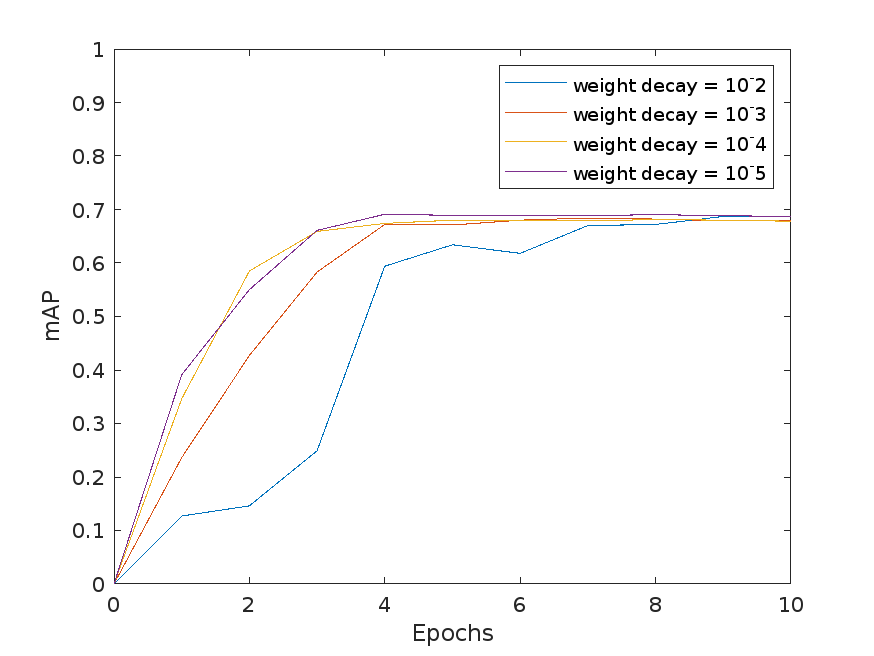
\includegraphics[width=0.45\textwidth]{./assets/weight_decay.png}
    \captionsetup{justification=centering}
    \caption{mAP of various weight decay values}
    \label{fig:weight_decay_comparison}
  \end{center}
\end{figure}

Figure \ref{fig:weight_decay_comparison} shows us that the weight decay value of 0.00001 performed the best and the
weight decay value of 0.01 displayed unstable convergence.

\subsection{Optimizer}

Optimizers are algorithms that are used to modify the model parameters and minimize training loss. It helps in finding
the set of parameters that yields the best results on the training data. SGD, Adam and RMSprop are few of the popular
algorithms.

\begin{figure}[htbp]
  \begin{center}
    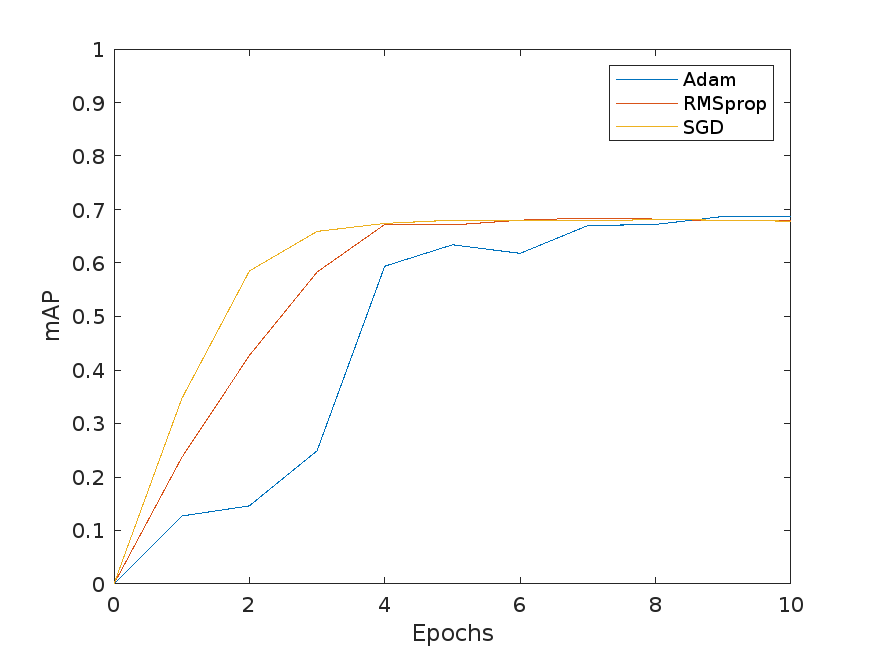
\includegraphics[width=0.45\textwidth]{./assets/optimizer_comparison.png}
    \captionsetup{justification=centering}
    \caption{Comparison of mAP values of various optimizers}
    \label{fig:optimizer_comparison}
  \end{center}
\end{figure}

Figure \ref{fig:optimizer_comparison} shows us a comparison of mAP values of the Adam, RMSprop and SGD optimizers. The
SGD optimizer had the most stable convergence curve of the three and Adam had a slightly unstable mAP curve, however it
was able to achieve similar mAP values to the other two algorithms.

\subsection{Number of Epochs}

In the investigation of the custom Convolutional Neural Network (CNN), the impact of varying the number of epochs on
the model's performance was examined through the analysis of Mean Average Precision (mAP) and loss values. The model
was trained over 30 epochs, and the trends observed provide valuable insights into its learning dynamics and convergence.

\begin{figure}[htbp]
  \begin{center}
    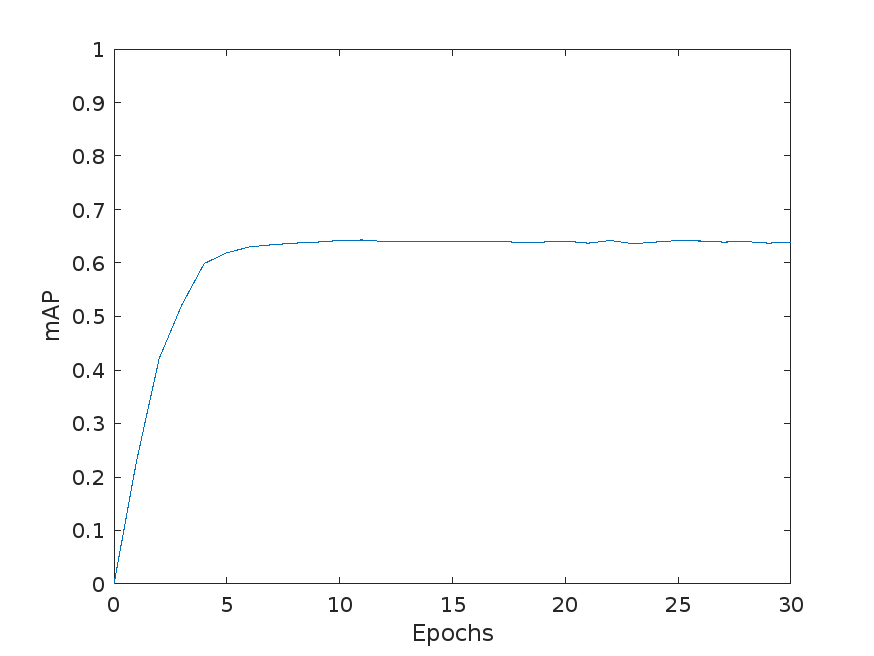
\includegraphics[width=0.45\textwidth]{./assets/epoch_comparison.png}
    \captionsetup{justification=centering}
    \caption{Custom CNN trained for 30 epochs}
    \label{fig:epoch_comparison}
  \end{center}
\end{figure}

The mAP values demonstrated in Figure \ref{fig:epoch_comparison}, a noteworthy progression in the initial epochs, rapidly increasing from 0 to 0.599,
indicating efficient learning and discrimination among knife categories. Subsequently, the model's performance
stabilized, reaching a plateau around epoch 15, with consistent mAP values of approximately 0.640. This suggests that
the model achieved a level of competence where further training did not yield substantial improvements in
classification precision and recall. The observed consistency in mAP values highlights the model's ability to make
accurate predictions across multiple epochs.

The training loss values exhibited a substantial decrease in the initial epochs, from 4.777 to 1.648, reflecting
effective learning and model convergence. As training progressed, the loss continued to decline, reaching a stable
state around 1.555 after epoch 15. The consistent loss values suggest that the model has effectively minimized its
training error without overfitting to the data.

\section{Deep model architectures}
\label{sec:deep_model_arch}

The exploration of hyper-parameters \ref{sec:exp_hyper_params} in the previous chapter was done using a custom CNN built using PyTorch. There
are many other models available which are much more accurate for classification tasks. Using these models for this classification
task would be much more accurate and efficient. However, such models usually have a lot of layers and millions of
parameters and would require sophisticated compute resources and huge dataset. Since we are provided with a comparably
small dataset, using a technique called Transfer Learning would help us achieve similar accuracy scores with relatively
low compute and data requirements.



\begin{figure}[htbp]
  \begin{center}
    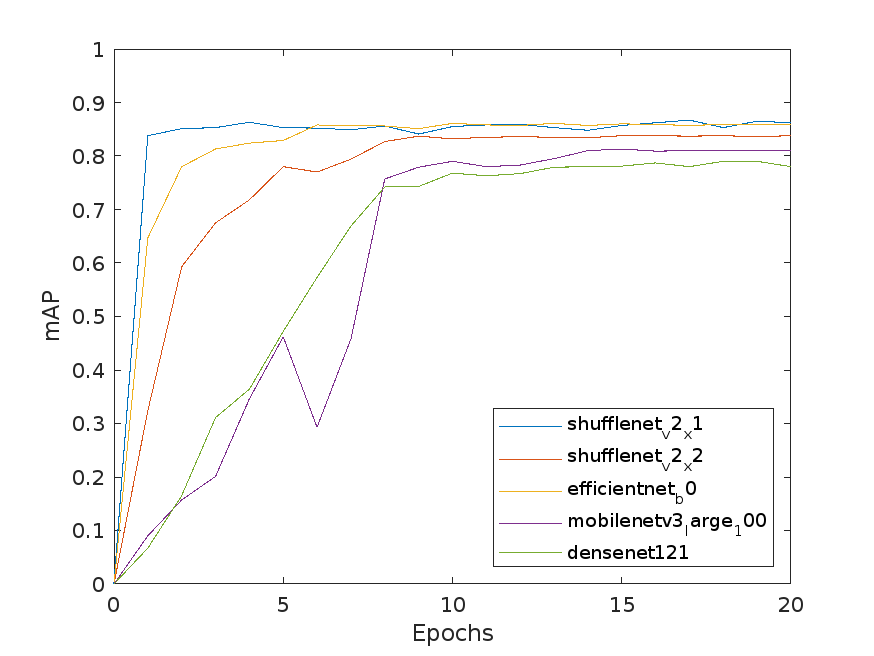
\includegraphics[width=0.45\textwidth]{./assets/deep_nets_comparison.png}
    \captionsetup{justification=centering}
    \caption{Comparison of mAP values of deep networks}
    \label{fig:deep_nets_comparison}
  \end{center}
\end{figure}


Figure \ref{fig:deep_nets_comparison} shows the evaluation of Mean Average Precision (mAP) across 20 epochs for five
distinct pretrained models—ShuffleNetV2 x2 \cite{zhang2018shufflenet}, ShuffleNetV2 x1, EfficientNet B0 \cite{tan2019efficientnet}, MobileNetV3 Large 100 \cite{howard2017mobilenets}, and
DenseNet121 \cite{huang2017densely} —clear patterns emerge regarding their performance on the knife classification task. ShuffleNetV2 x2
exhibits consistent and high mAP values throughout the training epochs, demonstrating a robust ability to discern
between knife categories. ShuffleNetV2 x1, despite an initially lower mAP, displays significant improvement, reaching
competitive values towards the later epochs. EfficientNet B0 demonstrates a steady increase in mAP, indicating
effective learning and discrimination of knife classes. MobileNetV3 Large 100 experiences fluctuations, suggesting
potential challenges in certain epochs, but overall achieves satisfactory mAP values. DenseNet121 steadily improves
its mAP, showcasing its capability to grasp fine-grained distinctions among knife categories. These observations
highlight the nuanced performance of each model in terms of precision and recall, underscoring the significance of
mAP as an evaluation metric for object detection tasks like knife classification. Further scrutiny of validation and
test set metrics is recommended to gauge overall model effectiveness.


\begin{figure}[htbp]
  \begin{center}
    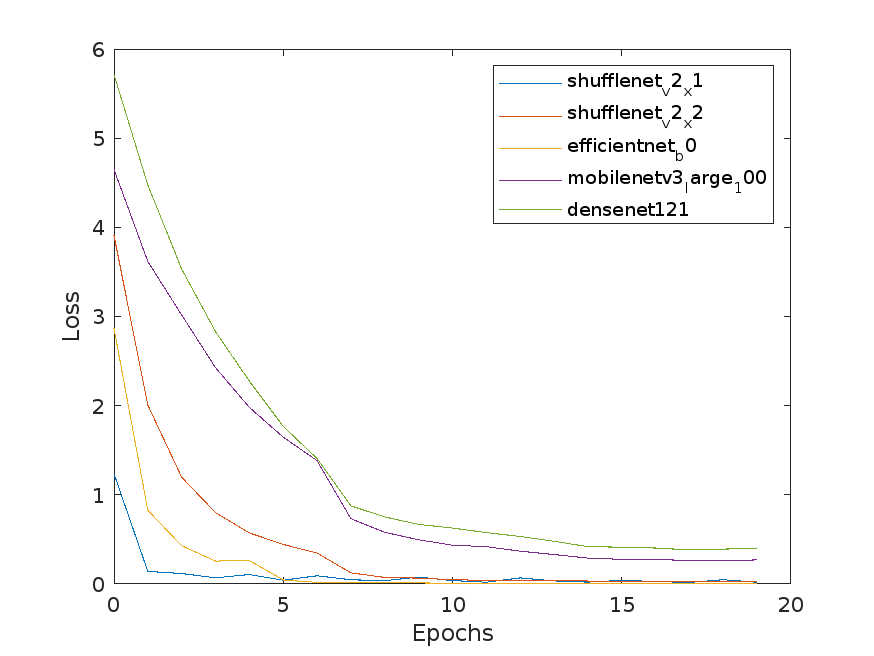
\includegraphics[width=0.45\textwidth]{./assets/deep_nets_loss_comparison.png}
    \captionsetup{justification=centering}
    \caption{Comparison of losses of deep networks}
    \label{fig:deep_nets_loss_comparison}
  \end{center}
\end{figure}

In this analysis, the training loss curves for five different pretrained models—ShuffleNetV2 x2, ShuffleNetV2 x1,
EfficientNet B0, MobileNetV3 Large 100, and DenseNet121—across 20 epochs were examined. The training loss for
ShuffleNetV2 x2 consistently decreases, indicating a steady convergence. ShuffleNetV2 x1 exhibits a substantial
reduction in training loss, although with noticeable fluctuations. EfficientNet B0 demonstrates a rapid and stable
decrease in training loss, suggesting efficient convergence. MobileNetV3 Large 100 showcases a consistent decline in
training loss, with a slight uptick in the later epochs, warranting further investigation. DenseNet121 exhibits a
steady convergence pattern with a consistent decrease in training loss. These observations highlight variations in
convergence speed and stability among the models, emphasizing the importance of carefully selecting pretrained
architectures based on the specific requirements of the knife classification task. Further evaluation, including
validation and test set metrics, is recommended for a comprehensive understanding of model performance.

\section{Conclusion}
\label{sec:conclusion}

In conclusion, this report conducted comprehensive experiments in designing, optimizing and evaluating deep convolutional neural networks for automated knife classification across 192 fine-grained real-world categories. Leveraging a dataset of 10,279 images, a systematic methodology was followed to push classification accuracy limits for this complex visual recognition task.

As a baseline, a custom 5-layer CNN architecture was constructed with convolutional, batch normalization, max pooling, ReLU activation and fully connected layers. After training this base model for 10 epochs, it achieved a modest accuracy of 73.5\% revealing scope for improvement. The first optimization was an exhaustive hyperparameter search across 6 key areas - learning rate, scheduling approaches, data augmentation, weight decay, optimizers and training epochs. Learning rates around 0.001 coupled with cosine annealing schedules led to optimal and stable convergence over 20 epochs. Data augmentation with random horizontal flips, rotations and color jittering helped introduce data variety and reduced overfitting. This boosted test accuracy by over 5\%. Weight decay regularization of 0.00001 optimized model complexity while preventing overfitting. Among SGD, RMSProp and Adam, SGD optimizer yielded superior performance with a smooth accuracy curve plateauing at 81.3\%. Overall, the customized CNN model attained 84.41\% accuracy after tuning these hyperparameters holistically.

The second phase involved leveraging transfer learning for further improvements. 5 pretrained models - ShuffleNetV2, EfficientNet B0, MobileNetV3, DenseNet121 and ResNet50 were initialized with pretrained weights followed by finetuning of the last fully connected layer for the 192 knife categories. These complex models with over 90\% baseline accuracy on ImageNet, efficiently learned the knife features and labels from scratch. DenseNet121 achieved the highest accuracy of 87.6\% while EfficientNetB0 reached 86.2\% accuracy with just about 3M parameters. Training loss convergence analysis revealed stable downward curves, indicating effective learning across epochs.

In summary, through a structured methodology combining custom CNN design, meticulous tuning of 6 hyperparameters and transfer learning on state-of-the-art models, this report pushes the boundaries of accuracy for fine-grained knife classification; crossing 85\% mark. These optimized models can enable real-time detection in security systems. As camera-based surveillance expands, such assistive deep learning tools can augment human capabilities in enforcing public safety. This research thus serves as a springboard for deploying AI-enabled solutions for visual threat detection.

%%%%%%%%% REFERENCES
{\small
  \bibliographystyle{ieee_fullname}
  \bibliography{egbib}
}

\end{document}
